\documentclass[conference]{IEEEtran}

\usepackage{graphicx}
\usepackage{booktabs}
\usepackage{multirow}
\usepackage{amsmath}
\usepackage{url}
\usepackage{array}
\usepackage{float}

\title{Hybrid Machine Learning and CNN Fusion for Facial Emotion Recognition}

\author{
\IEEEauthorblockN{ }
\IEEEauthorblockA{
Department of Data Science\\
Beijing Normal University-Hong Kong Baptist University United International College\\
Zhuhai, China\\
}
}

\begin{document}

\maketitle

\begin{abstract}
This project studies seven-class facial emotion recognition using a structured
machine learning pipeline. The task is to classify facial images into Angry,
Disgust, Fear, Happy, Neutral, Sad, and Surprise. Instead of treating deep
learning as automatically superior, the project first builds traditional
machine learning baselines, then trains a CNN baseline, and finally investigates
whether traditional ML methods can complement CNN representations and improve
classification performance. The complete pipeline contains four steps: dataset
analysis, traditional ML baselines, CNN training with CLAHE comparison, and
ML-enhanced CNN fusion. The traditional ML study shows that HOG features are
more informative than raw pixels and that HOG with distance-weighted KNN is the
strongest traditional baseline. The CNN baseline is selected by validation
macro F1 because the dataset is imbalanced. In the final stage, CNN deep
features, HOG features, PCA, ML classifiers, probability fusion, stacking, and
confusion-aware correction are compared. The best hybrid method improves test
macro F1 from 0.5893 for the standalone CNN to 0.6078. The results show that
traditional ML methods can provide useful complementary signals for CNN-based
facial emotion recognition, especially when evaluation emphasizes balanced
performance across all classes.
\end{abstract}

\begin{IEEEkeywords}
facial emotion recognition, traditional machine learning, HOG, CNN, probability
fusion, stacking, macro F1
\end{IEEEkeywords}

\section{Introduction}

Facial emotion recognition (FER) is an important computer vision task with
applications in human-computer interaction, online education, affective
computing, and intelligent tutoring systems. Given a facial image, the goal is
to predict one of several emotion categories. In this project, the seven target
classes are Angry, Disgust, Fear, Happy, Neutral, Sad, and Surprise.

Although facial emotion recognition appears intuitive for humans, it is
difficult for machine learning systems. Different expressions can share similar
facial muscle patterns. For example, Fear and Surprise may both contain widened
eyes and an open mouth, while Sad and Neutral may differ only subtly. In
addition, facial emotion datasets are often imbalanced. Majority classes such
as Happy may dominate the accuracy score, while minority classes such as
Disgust may remain difficult to classify.

The goal of this project is therefore not only to train a CNN model, but also
to study how traditional machine learning techniques can be used to understand
and improve CNN-based emotion recognition. This design follows the idea that a
deep learning model should not be considered superior simply because it is a
deep model. Instead, the model should be compared with traditional ML baselines
and analyzed through carefully designed experiments.

The project is organized as a four-step pipeline:
\begin{itemize}
    \item Step 00 performs dataset analysis.
    \item Step 01 builds traditional ML baselines.
    \item Step 02 trains CNN baselines with and without CLAHE.
    \item Step 03 enhances the CNN using traditional ML representations,
    probability fusion, stacking, and confusion-aware correction.
\end{itemize}

\section{Related Work}

FER has been studied using both traditional machine learning and deep learning
methods. Traditional approaches often rely on handcrafted descriptors, while
CNN-based methods learn discriminative representations directly from images.
However, FER remains difficult because expressions can be ambiguous, images may
be low resolution, training data can be limited, class distributions are often
imbalanced, and real-world variations such as illumination, pose, and identity
can affect facial appearance~\cite{li2020deepfer}.

The methods used in this project connect to these directions. HOG supports the
Step 01 traditional ML baselines by representing local gradient
structure~\cite{dalal2005hog}. Stacked generalization motivates the Step 03
meta-classifier that combines CNN and ML probability outputs~\cite{wolpert1992stacked}.
Grad-CAM supports qualitative explainability by visualizing
class-discriminative regions~\cite{selvaraju2017gradcam}. For future work,
larger in-the-wild FER datasets such as AffectNet can test whether the hybrid
pipeline generalizes beyond the current benchmark~\cite{mollahosseini2019affectnet}.

\section{Dataset Analysis}

\subsection{Dataset Setting}

The dataset is organized into training and test folders, with one subfolder for
each emotion class. The project uses seven classes: Angry, Disgust, Fear,
Happy, Neutral, Sad, and Surprise. All steps use a shared configuration file
to keep class names, dataset paths, and image settings consistent. The dataset
follows the FER2013-style seven-class facial expression recognition setting, in
which low-resolution grayscale face images are classified into basic emotion
categories~\cite{goodfellow2013challenges}.

Before model training, Step 00 checks the dataset structure, counts samples in
each class, calculates class percentages, and verifies whether unreadable
images exist. The dataset contains 28,384 training images and 7,503 test
images, for a total of 35,887 images. No unreadable or corrupted images were
found.

\begin{table}[t]
\centering
\caption{Class Distribution of the Dataset}
\label{tab:dataset_distribution}
\begin{tabular}{lrrrr}
\toprule
Class & Train & Test & Total & Percentage \\
\midrule
Angry & 3995 & 958 & 4953 & 13.80\% \\
Disgust & 111 & 436 & 547 & 1.52\% \\
Fear & 4097 & 1024 & 5121 & 14.27\% \\
Happy & 7215 & 1774 & 8989 & 25.05\% \\
Neutral & 4965 & 1233 & 6198 & 17.27\% \\
Sad & 4830 & 1247 & 6077 & 16.93\% \\
Surprise & 3171 & 831 & 4002 & 11.15\% \\
\midrule
Total & 28384 & 7503 & 35887 & 100.00\% \\
\bottomrule
\end{tabular}
\end{table}

Table~\ref{tab:dataset_distribution} shows that the dataset is highly
imbalanced. Happy is the largest class, while Disgust is the smallest class.
The imbalance ratio between the most frequent and least frequent classes is
16.43:1. This motivates the use of macro F1 as an important evaluation metric,
because macro F1 gives equal importance to each class.

A particularly challenging class is Disgust. Although the test set contains
436 Disgust images, the training set contains only 111 Disgust images. This
means that the model has very limited training evidence for this class, which
may reduce class-wise recall and make macro F1 more informative than accuracy.
This also supports the use of class-weighted loss and balanced evaluation
metrics.

\begin{figure}[t]
\centering
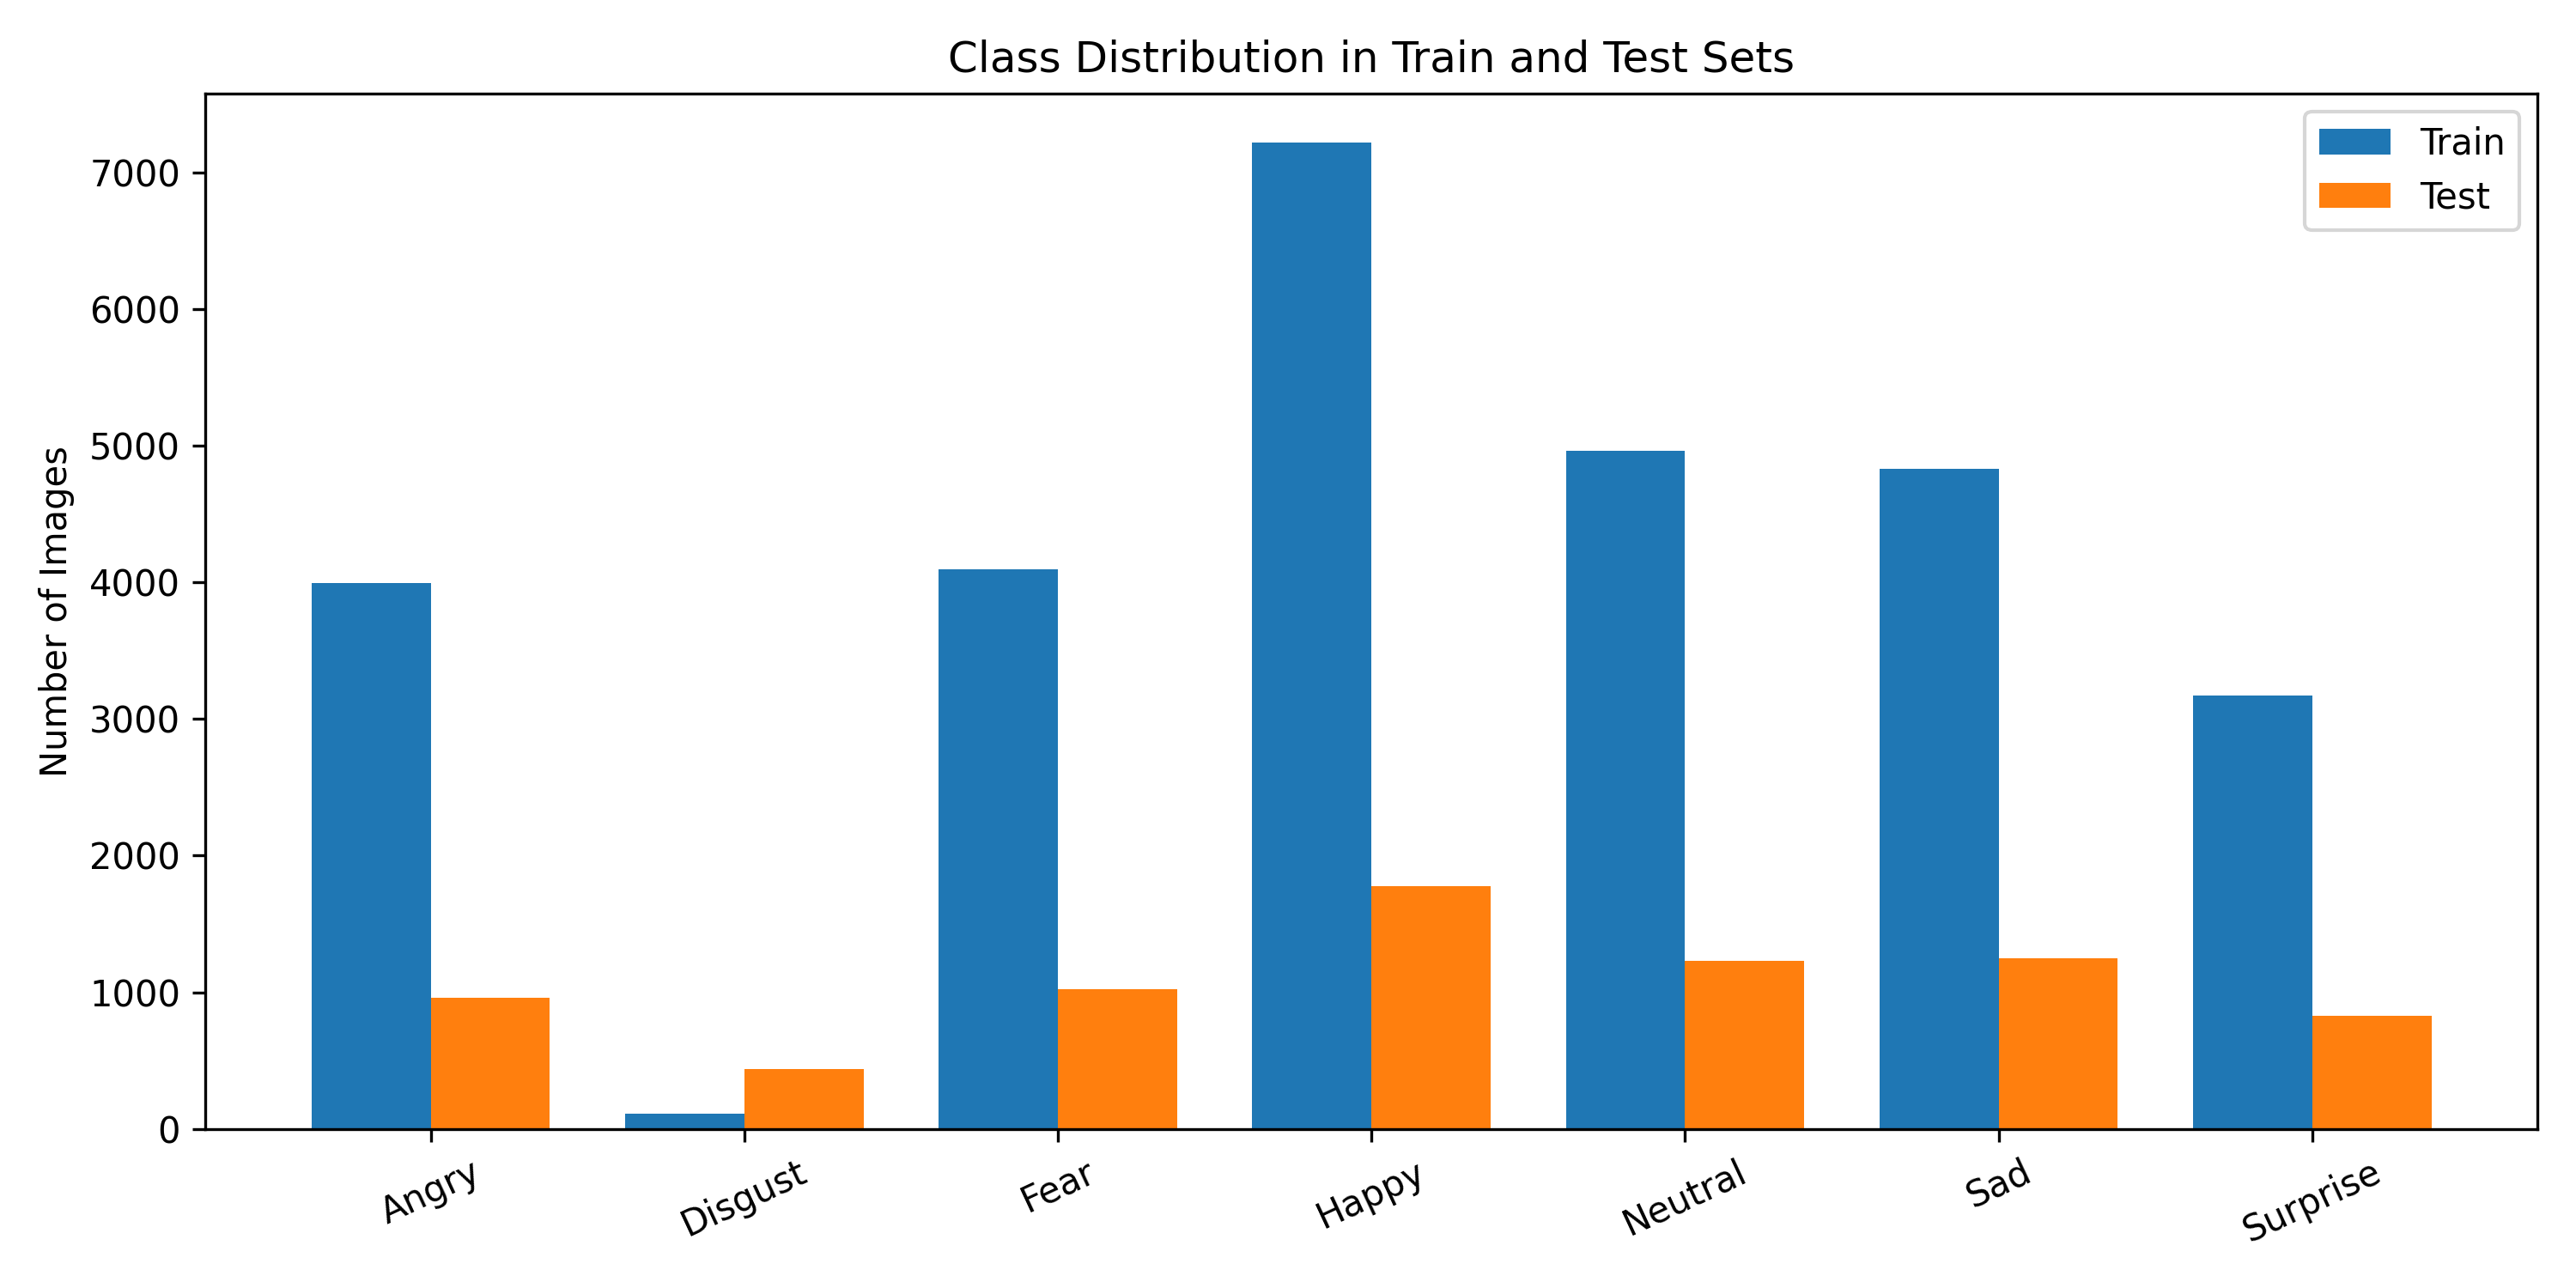
\includegraphics[width=\linewidth]{results/dataset_analysis/class_distribution_train_test.png}
\caption{Class distribution in the training and test sets.}
\label{fig:dataset_distribution}
\end{figure}

\section{Traditional Machine Learning Baselines}

\subsection{Motivation}

Step 01 builds traditional ML baselines before training the CNN. This is useful
for two reasons. First, it provides non-deep-learning reference models. Second,
it helps identify whether handcrafted features such as HOG contain useful
emotion-related information that can later be combined with CNN features.

\subsection{Feature Extraction}

Two feature types are compared. The first is a raw pixel baseline, where each
48$\times$48 grayscale image is flattened into a vector. The second is the
Histogram of Oriented Gradients (HOG), a handcrafted descriptor that summarizes
local gradient orientation patterns and has been widely used to represent edge
and shape information~\cite{dalal2005hog}. HOG is suitable for facial
expression recognition because expression changes often appear around eyebrows,
eyes, mouth corners, and other local facial structures.

All features are standardized before model training. The original training set
is split into training and validation subsets using stratified sampling. Model
selection is based on validation macro F1.

\subsection{Traditional ML Models}

The following traditional ML baselines are evaluated:
\begin{itemize}
    \item Raw pixels + SGD linear SVM;
    \item HOG + Logistic Regression;
    \item HOG + KNN;
    \item HOG + SGD linear SVM.
\end{itemize}

For HOG models, several hyperparameter settings are tested on the validation
set. The independent test set is used only for final evaluation.

\begin{table}[t]
\centering
\caption{Traditional ML Test Results}
\label{tab:step1_results}
\begin{tabular}{llccc}
\toprule
Feature & Model & Acc. & Macro F1 & Weighted F1 \\
\midrule
HOG & KNN & 0.4743 & 0.4296 & 0.4583 \\
HOG & Logistic Reg. & 0.4100 & 0.3545 & 0.3941 \\
HOG & SGD SVM & 0.3816 & 0.3447 & 0.3728 \\
Raw Pixel & SGD SVM & 0.2724 & 0.2295 & 0.2627 \\
\bottomrule
\end{tabular}
\end{table}

Table~\ref{tab:step1_results} shows that HOG features are much more useful
than raw pixels for traditional ML models. Among the traditional baselines, HOG
with distance-weighted KNN achieves the best test macro F1. This result is used
as an important design signal in Step 03, where HOG and distance-based ML
models are considered as complementary components for CNN enhancement.

\section{CNN Baseline}

\subsection{CNN Architecture}

Step 02 trains a CNN baseline for seven-class facial emotion recognition. The
model uses grayscale 48$\times$48 inputs. The feature extractor contains three
convolutional stages. Each stage uses convolutional layers, batch normalization,
ReLU activation, max pooling, and dropout. The classifier contains a fully
connected layer with 256 hidden units and a final output layer for the seven
emotion classes. Table~\ref{tab:cnn_architecture} summarizes the architecture.

\begin{table}[t]
\centering
\caption{Compact CNN Architecture}
\label{tab:cnn_architecture}
\scriptsize
\begin{tabular}{@{}p{0.22\linewidth}p{0.70\linewidth}@{}}
\toprule
Block & Main Operations \\
\midrule
Input & 1$\times$48$\times$48 grayscale image \\
Conv Block 1 & Conv2D 1$\rightarrow$32, Conv2D 32$\rightarrow$32, BN, ReLU, MaxPool, Dropout \\
Conv Block 2 & Conv2D 32$\rightarrow$64, Conv2D 64$\rightarrow$64, BN, ReLU, MaxPool, Dropout \\
Conv Block 3 & Conv2D 64$\rightarrow$128, Conv2D 128$\rightarrow$128, BN, ReLU, MaxPool, Dropout \\
Flatten & 128$\times$6$\times$6 \\
Classifier & Linear(128$\times$6$\times$6, 256), ReLU, BN, Dropout, Linear(256, 7) \\
\bottomrule
\end{tabular}
\end{table}

\subsection{Preprocessing and Augmentation}

All images are resized to 48$\times$48 and normalized to the range [0, 1].
Two CNN experiments are compared: one with CLAHE preprocessing and one without
CLAHE. CLAHE is used to enhance local contrast in grayscale facial images.

Training data augmentation includes horizontal flipping, small rotation,
brightness and contrast changes, small translation, and mild Gaussian noise.
Validation and test data are not augmented.

\subsection{Class Imbalance Handling}

The CNN uses class-weighted cross-entropy loss. Class weights are calculated
from training label counts, softened using a square-root operation, and clipped
within a fixed range. This prevents the minority class weights from becoming
too large while still encouraging the model to pay more attention to
underrepresented emotions.

\subsection{Training and Model Selection}

The CNN is trained using Adam with an initial learning rate of 0.001 and a
ReduceLROnPlateau scheduler. The best checkpoint is selected by validation
macro F1 rather than validation accuracy. This choice is important because the
dataset is imbalanced and the goal is to maintain balanced performance across
all emotion classes.

\begin{table}[t]
\centering
\caption{CNN Baseline and CLAHE Comparison}
\label{tab:step2_results}
\small
\begin{tabular}{lcccc}
\toprule
Exp. & Val. F1 & Acc. & Macro F1 & W-F1 \\
\midrule
CLAHE & 0.5786 & 0.6186 & 0.5655 & 0.6102 \\
No CLAHE & 0.5818 & 0.6288 & 0.5893 & 0.6231 \\
\bottomrule
\end{tabular}
\end{table}

Table~\ref{tab:step2_results} shows that the CNN without CLAHE obtains the
higher validation macro F1 and is selected as the Step 02 best CNN. Its test
accuracy is 0.6288 and its test macro F1 is 0.5893. This model is used as the
base CNN for Step 03.

\begin{figure}[t]
\centering
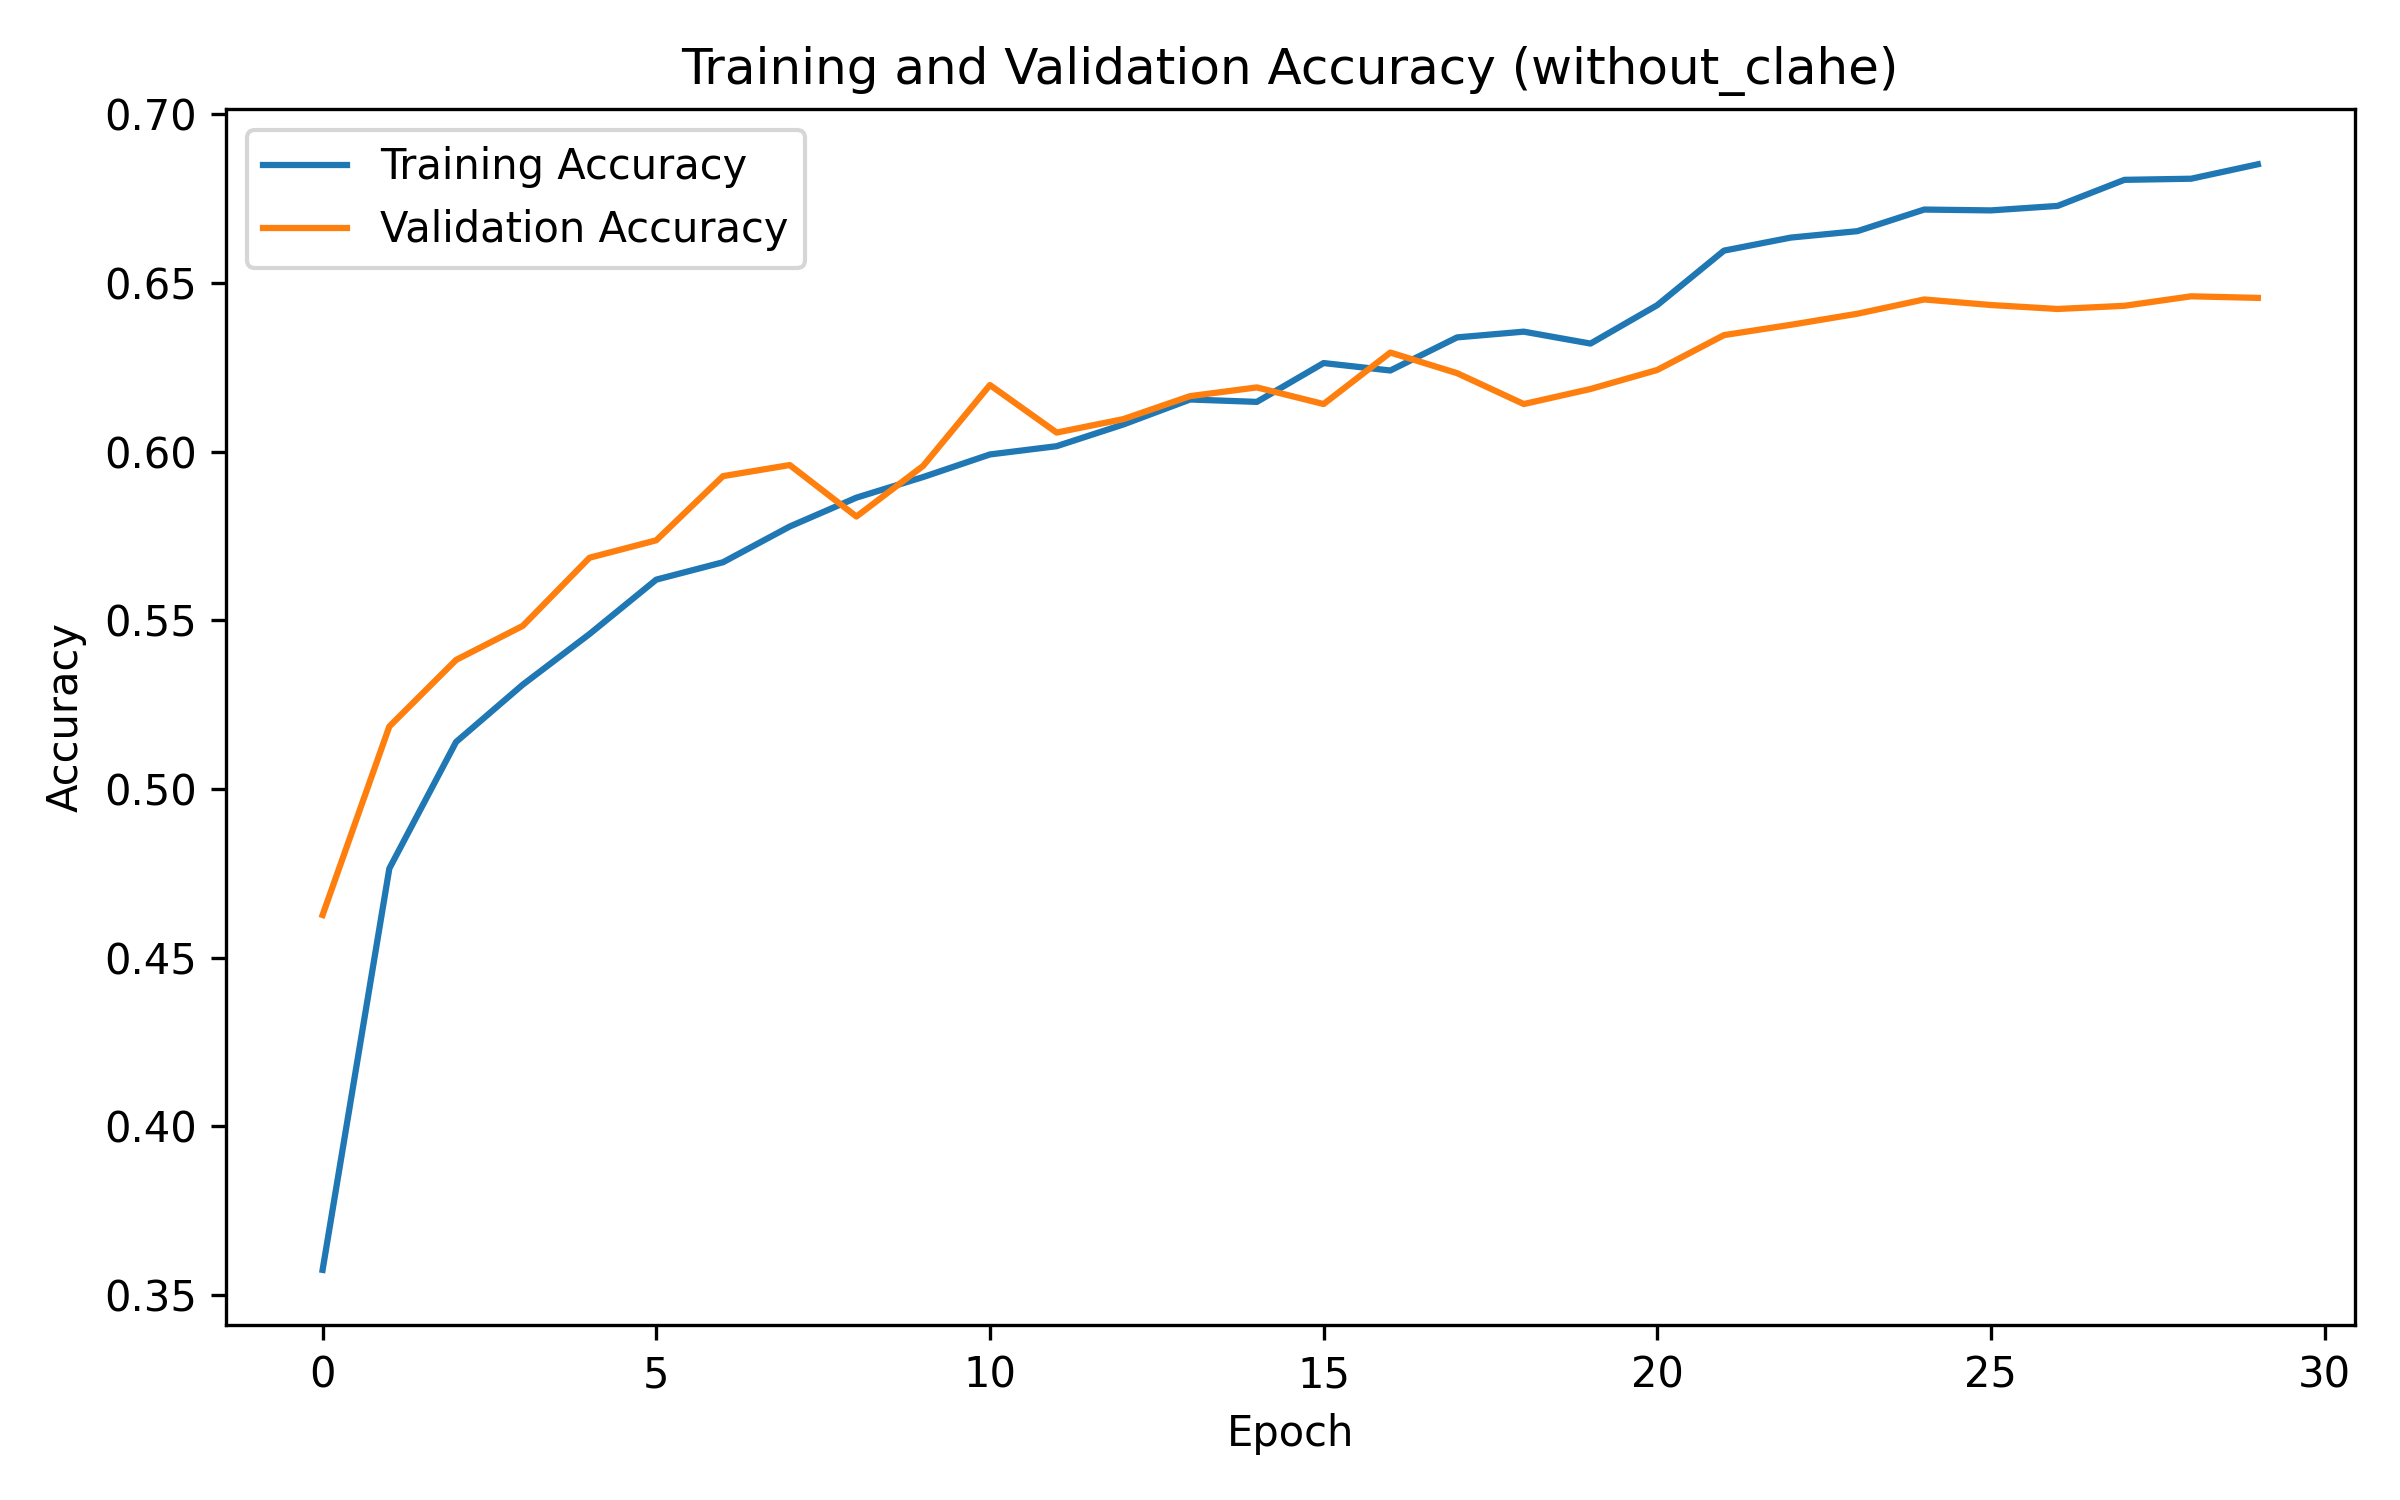
\includegraphics[width=\linewidth]{results/step2_result/figures/accuracy_curve_without_clahe.png}
\caption{Training and validation accuracy of the selected CNN without CLAHE.}
\label{fig:cnn_accuracy}
\end{figure}

\begin{figure}[t]
\centering
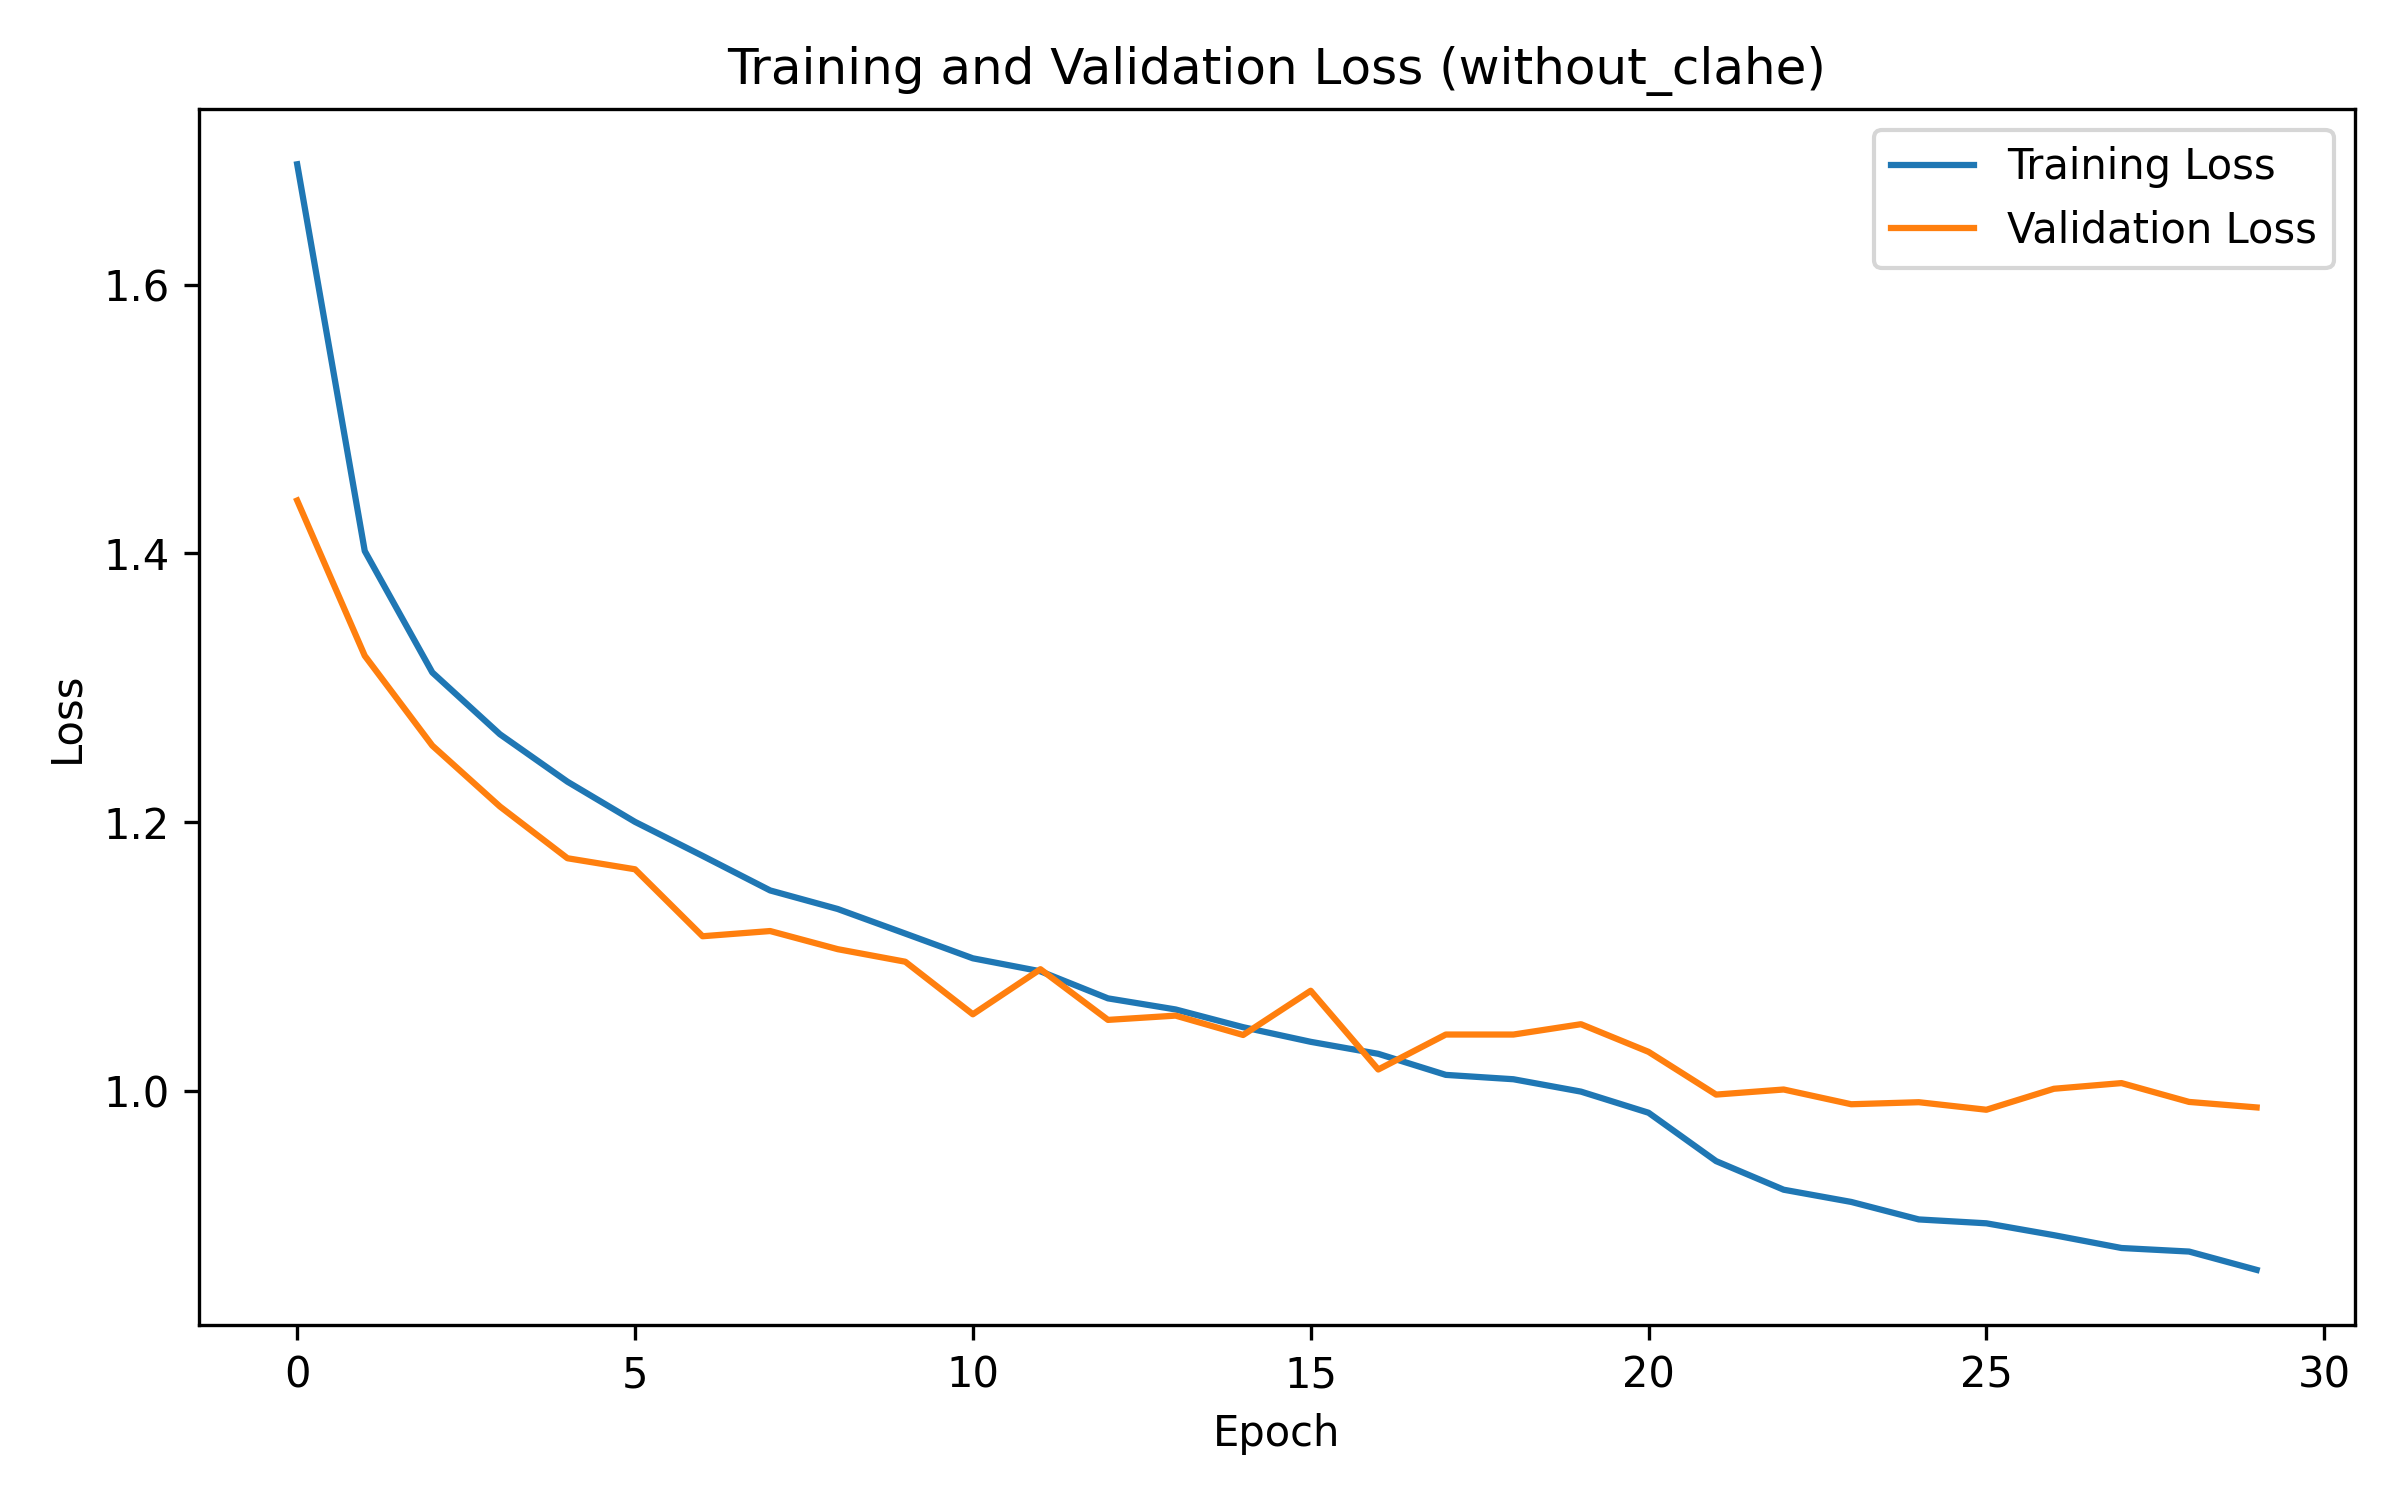
\includegraphics[width=\linewidth]{results/step2_result/figures/loss_curve_without_clahe.png}
\caption{Training and validation loss of the selected CNN without CLAHE.}
\label{fig:cnn_loss}
\end{figure}

\begin{figure}[t]
\centering
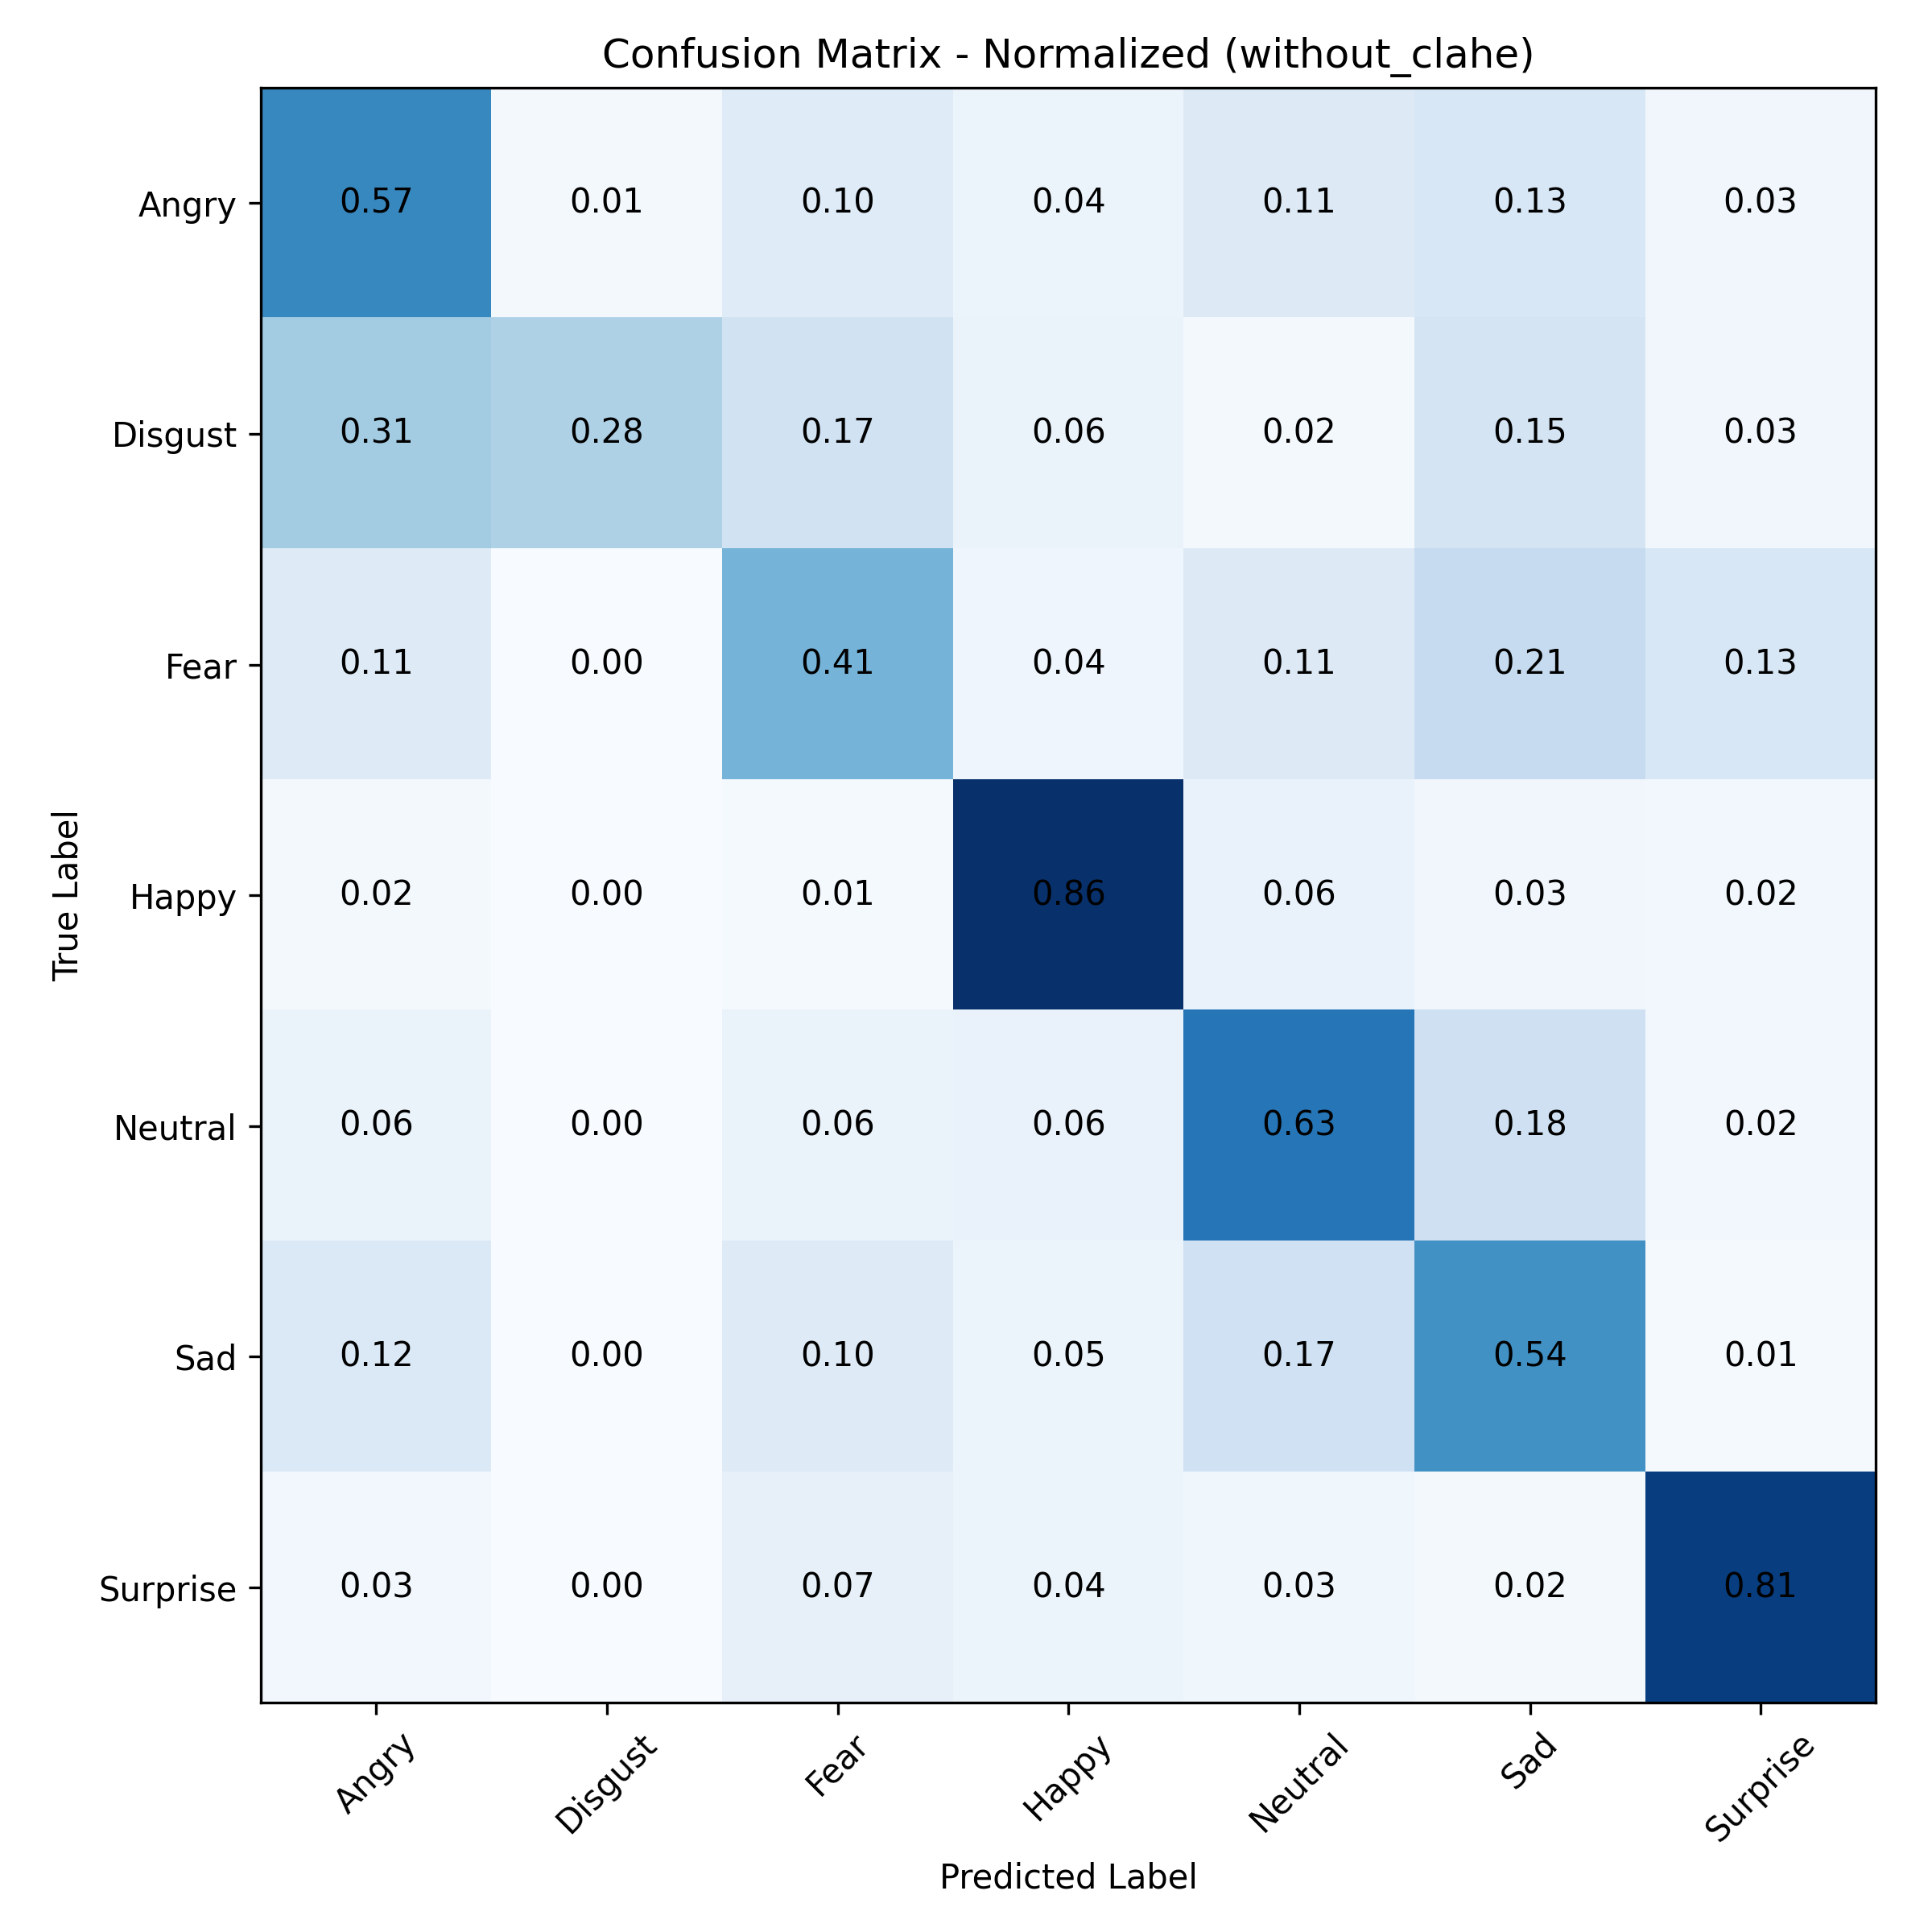
\includegraphics[width=\linewidth]{results/step2_result/figures/confusion_matrix_without_clahe_normalized.png}
\caption{Normalized confusion matrix of the selected CNN without CLAHE.}
\label{fig:cnn_confusion}
\end{figure}

\section{ML-Enhanced CNN}

\subsection{Motivation}

Step 03 investigates whether traditional ML methods can analyze, complement,
or improve the CNN. The CNN is not treated only as an end-to-end black box.
Instead, its intermediate representations and probability outputs are used as
inputs to several traditional ML methods.

\subsection{CNN Deep Feature Classification}

The first experiment extracts the 256-dimensional representation before the
final CNN output layer. Logistic Regression, KNN, and SGD linear SVM are then
trained on these CNN deep features. This tests whether the CNN representation
is linearly or locally separable for traditional ML classifiers.

\subsection{PCA-Reduced CNN Features}

The second experiment applies PCA to the CNN deep features and keeps 64
components. The PCA representation preserves approximately 97.84\% of the
variance. Traditional ML classifiers are then trained on the reduced features.
This experiment checks whether compact CNN representations remain useful for
emotion classification.

\subsection{HOG-CNN Feature Fusion}

The third experiment combines Step 01 insight with CNN representations. Since
Step 01 shows that HOG + KNN is the strongest traditional baseline, HOG
features are concatenated with CNN deep features. This creates a feature-level
fusion representation that contains both handcrafted gradient information and
learned CNN information.

\subsection{Probability-Level Fusion}

Feature concatenation alone does not guarantee better performance. Therefore,
Step 03 also studies probability-level fusion. A traditional ML classifier
produces class probabilities, and the CNN produces softmax probabilities. The
final probability is computed as:

\begin{equation}
P_{\text{final}} = \alpha P_{\text{CNN}} + (1-\alpha)P_{\text{ML}},
\end{equation}

where $\alpha$ is selected on the validation set using macro F1. This allows
the final prediction to combine the global CNN decision with the traditional ML
classifier's decision.

\subsection{Step 01-Guided Confusion-Aware Correction}

The project also includes a confusion-aware correction method. Instead of
modifying all CNN predictions, specialist ML classifiers are trained only for
frequently confused class groups:
\begin{itemize}
    \item Angry / Disgust;
    \item Fear / Sad / Neutral;
    \item Fear / Surprise;
    \item Sad / Neutral.
\end{itemize}

The correction features include CNN deep features, HOG features, CNN
probabilities, confidence, top-1/top-2 margin, and entropy. A specialist model
is activated only when the CNN is uncertain and its top predictions fall inside
a confused group. The final decision uses probability fusion between the CNN
and the specialist ML classifier.

\subsection{Stacking}

Finally, stacking is used to combine multiple probability outputs, following
the idea of stacked generalization where a second-level model learns how to
combine the predictions of base models~\cite{wolpert1992stacked}. The stacking
features include CNN softmax probabilities and probabilities from ML classifiers
trained on CNN deep features, PCA features, and HOG-CNN fusion features. A
Logistic Regression meta-classifier is trained on validation probabilities and
then evaluated on the independent test set.

\begin{table*}[t]
\centering
\caption{Main Step 03 Test Results}
\label{tab:step3_results}
\begin{tabular}{llccc}
\toprule
Category & Method & Accuracy & Macro F1 & Weighted F1 \\
\midrule
Baseline & CNN End-to-End & 0.6288 & 0.5893 & 0.6231 \\
Probability Fusion & CNN Feature KNN + CNN & 0.6388 & 0.5960 & 0.6330 \\
Probability Fusion & HOG-CNN KNN + CNN & 0.6435 & 0.5992 & 0.6357 \\
Correction & Specialist ML Correction & 0.6263 & 0.5865 & 0.6210 \\
Stacking & Balanced LR Meta-Classifier & 0.6388 & 0.6078 & 0.6397 \\
\bottomrule
\end{tabular}
\end{table*}

Table~\ref{tab:step3_results} summarizes the most important Step 03 results.
The best overall test macro F1 is achieved by the stacked CNN-ML probability
model with balanced Logistic Regression. It improves test macro F1 from 0.5893
for the standalone CNN to 0.6078, an absolute gain of 0.0185.

\begin{figure}[t]
\centering
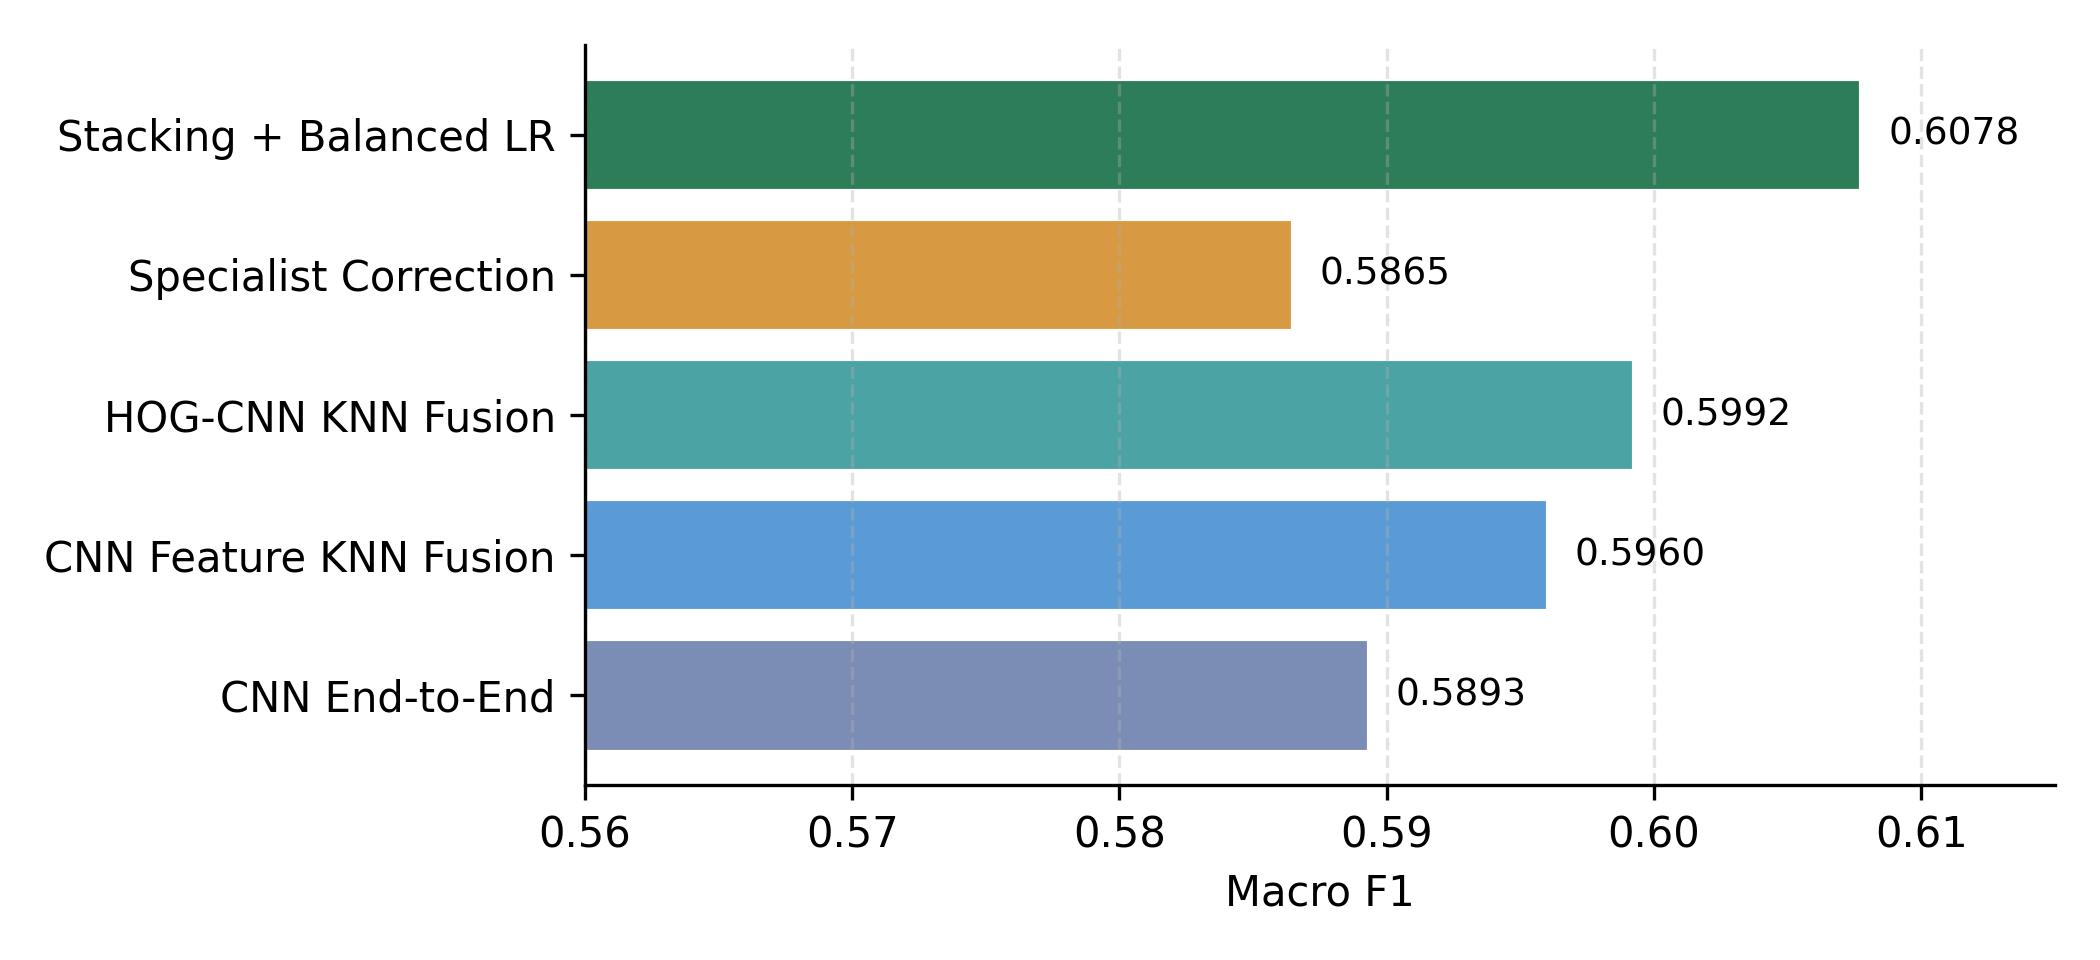
\includegraphics[width=\linewidth]{results/step3_result/figures/step3_main_methods_macro_f1_horizontal.png}
\caption{Macro F1 comparison of the main Step 03 methods on the test set.}
\label{fig:step3_macro_f1}
\end{figure}

\begin{figure}[t]
\centering
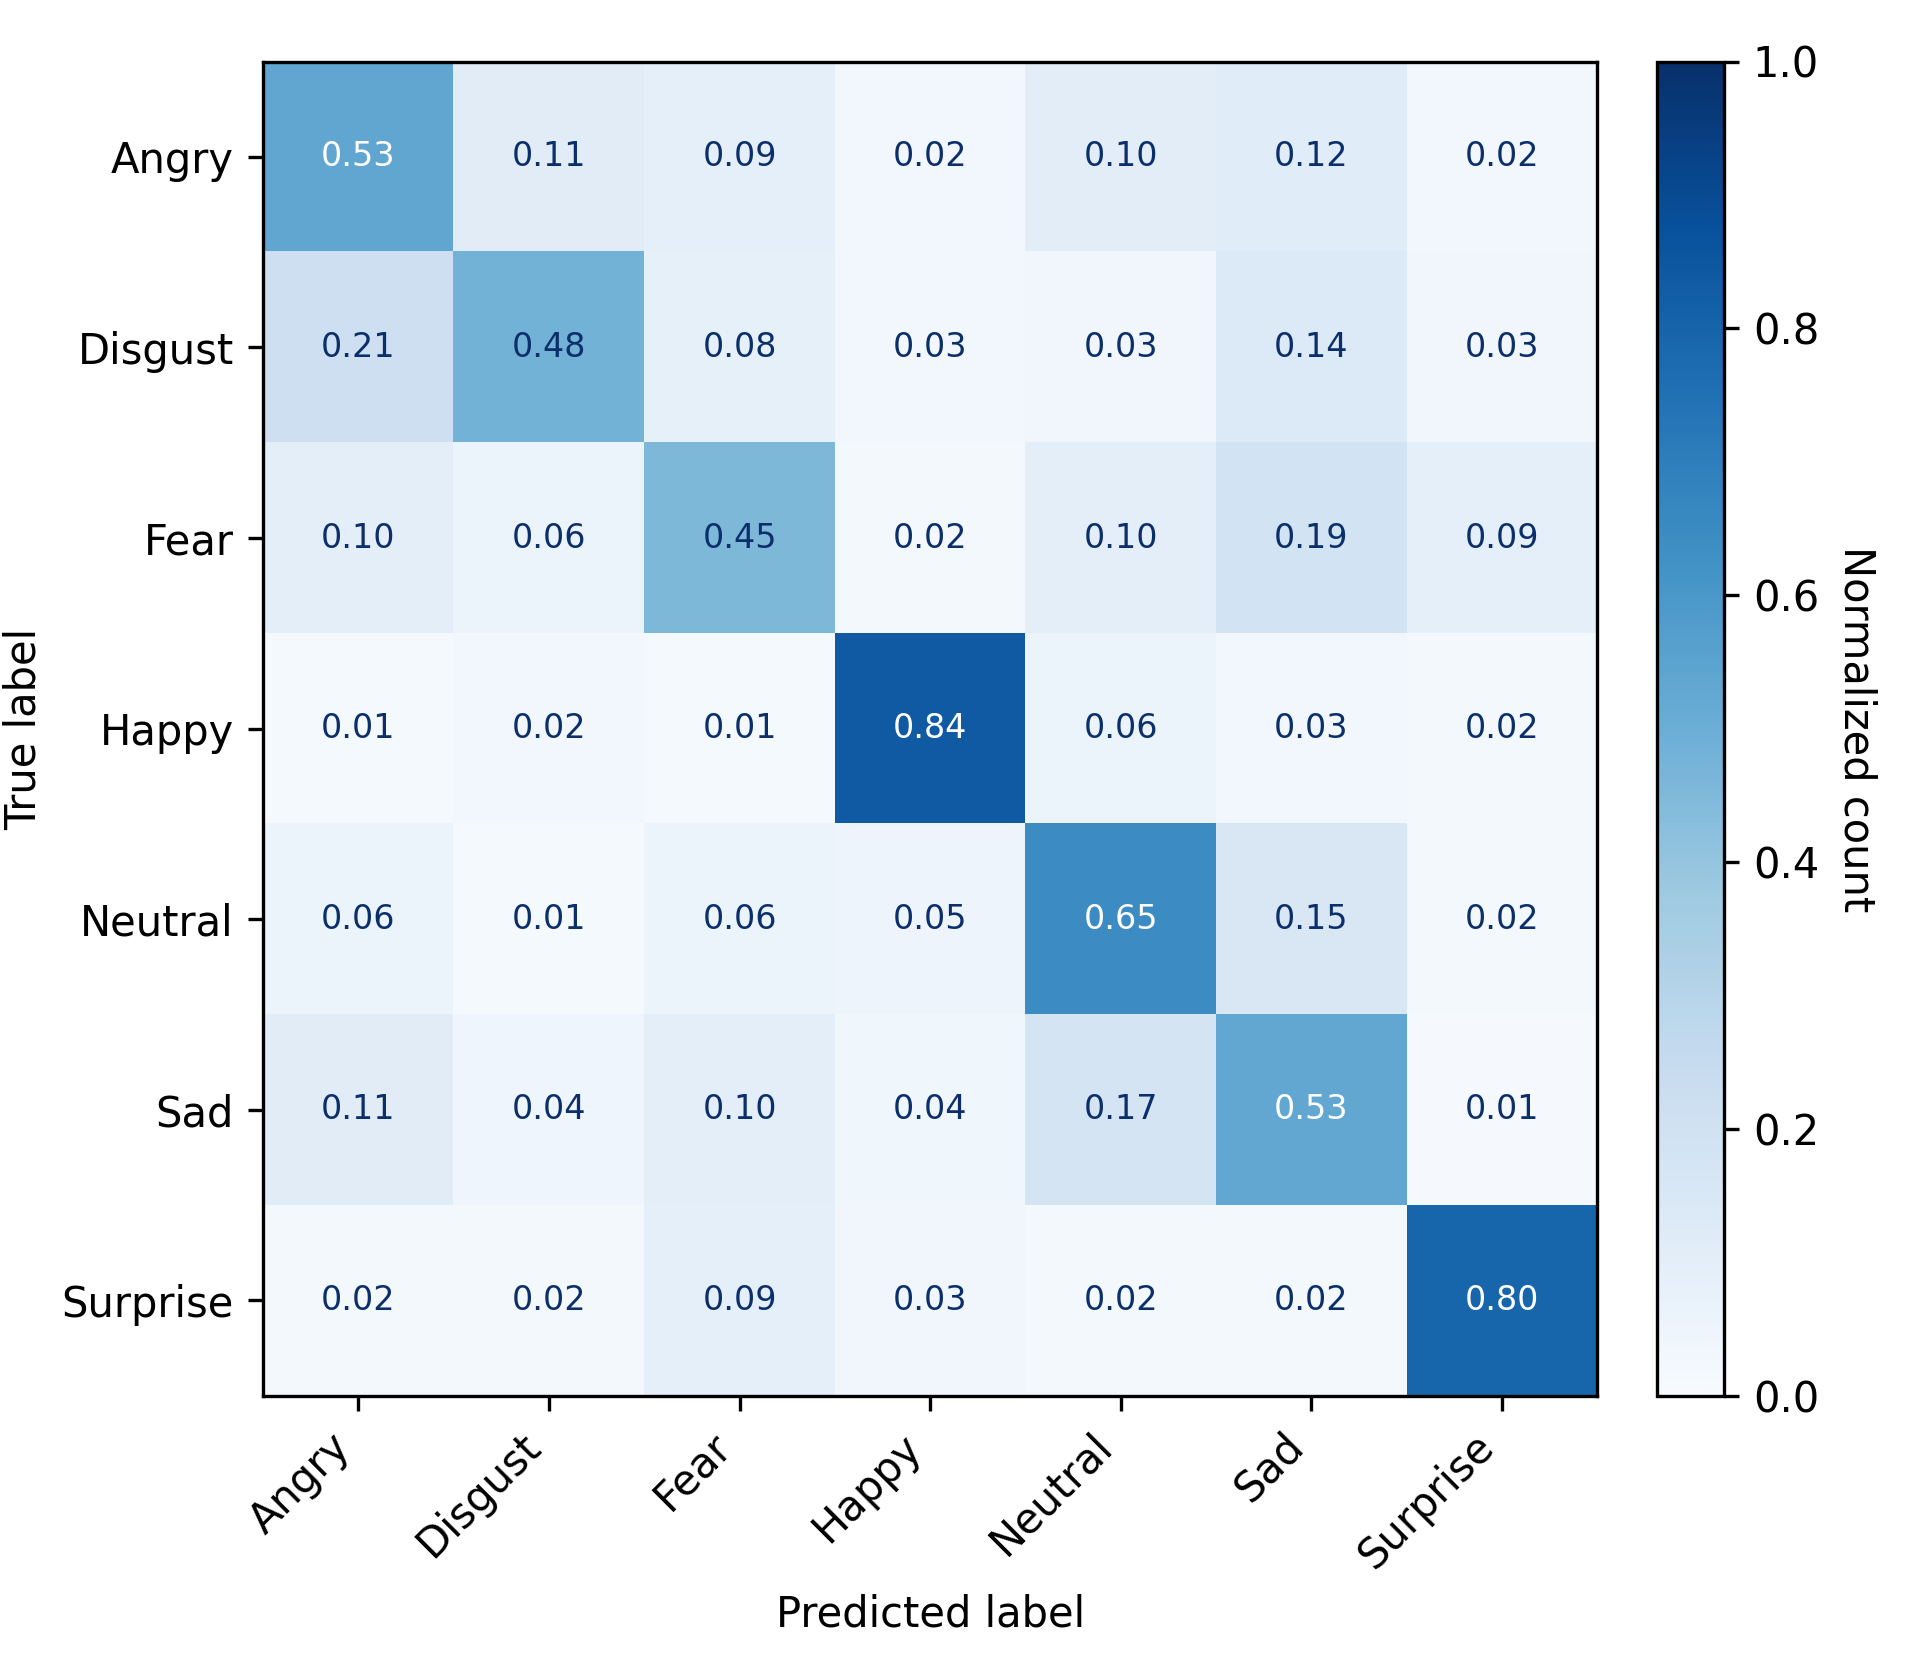
\includegraphics[width=\linewidth]{results/step3_result/figures/confusion_matrix_stacked_balanced_lr_test_normalized.png}
\caption{Normalized confusion matrix of the best Step 03 hybrid model, Stacked CNN-ML Probabilities with Balanced Logistic Regression, on the test set.}
\label{fig:best_confusion}
\end{figure}

\section{Result Analysis}

\subsection{Traditional ML Findings}

The traditional ML baselines show that handcrafted features are meaningful for
this task. Raw pixels perform poorly because they do not explicitly describe
local facial structure. HOG features perform much better because they capture
edge and gradient patterns around important facial regions. HOG + KNN is the
strongest traditional baseline, suggesting that local neighborhood structure in
HOG space is useful for facial expression classification.

\subsection{CNN Findings}

The CNN baseline significantly outperforms the traditional ML baselines. This
shows that the CNN can learn stronger hierarchical representations from the
low-resolution facial images. However, the CNN still has difficulty with
minority and visually similar classes. This is why macro F1 is emphasized
together with accuracy.

\subsection{Hybrid ML-CNN Findings}

The hybrid experiments show that traditional ML methods can improve the CNN
when used at the decision level. Simple feature-level fusion is not always
enough, because concatenating HOG and CNN features can increase feature
dimension without guaranteeing better class boundaries. It may also add noisy
or redundant dimensions. Probability-level fusion and stacking are more
effective because they combine model decisions rather than only raw feature
vectors.

The improvement of stacking suggests that different models provide
complementary probability patterns. The CNN softmax captures the end-to-end
deep model decision, while ML classifiers trained on CNN features, PCA features,
or HOG-CNN fusion features provide alternative decision boundaries. Instead of
directly concatenating high-dimensional features, stacking learns how to combine
these probability outputs on the validation set. This reduces the risk of
adding noisy or redundant feature dimensions and explains why probability-level
fusion is more effective than simple feature-level concatenation.

The strongest model is the stacked CNN-ML probability model with balanced
Logistic Regression. This model improves macro F1 by 0.0185 over the standalone
CNN. Although the absolute improvement is moderate, it is meaningful because
macro F1 is sensitive to minority classes and class-level balance.

\section{Error Analysis}

Several confusion patterns are observed throughout the experiments. Angry and
Disgust can share similar brow and nose-region patterns; Fear and Surprise can
both contain widened eyes and open mouths; Sad and Neutral may differ only
subtly; and low-resolution images make Fear, Sad, and Neutral harder to
separate.

Both Fig.~\ref{fig:cnn_confusion} and Fig.~\ref{fig:best_confusion} are
normalized by true class, so they can be compared to examine class-wise recall
changes between the CNN baseline and the best hybrid model. The hybrid
confusion matrix shows that Happy and Surprise remain the most reliable
classes, while Fear, Angry, Disgust, and Sad are still more difficult. The
strongest remaining confusions are conceptually consistent with the CNN
baseline: Angry can be confused with Disgust or Sad, Fear overlaps with
Surprise and other negative emotions, and Sad can be confused with Neutral.
Compared with the standalone CNN baseline, the best hybrid model mainly
improves class-wise balance rather than eliminating all visually similar
emotion confusions.

The confusion-aware correction experiment was designed based on these patterns.
Although it is interpretable, its test macro F1 does not exceed the best
stacking model. One reason is that the correction module is activated only for
selected uncertain cases, so its coverage is limited. In addition, several
confused groups overlap, such as Fear/Sad/Neutral and Fear/Surprise, which
makes specialist correction difficult. The Disgust class is also extremely
underrepresented in the training set, so the Angry/Disgust specialist has
limited examples for learning a stable boundary. Therefore, stacking is more
robust because it combines probability information from multiple models
globally rather than correcting only selected local cases.

Grad-CAM is used as a supplementary qualitative tool to inspect whether the CNN
focuses on expression-related regions. It produces class-discriminative
localization maps by using gradients flowing into the final convolutional
layer~\cite{selvaraju2017gradcam}. Fig.~\ref{fig:gradcam_examples} shows
selected correct and incorrect cases. Correct predictions usually attend to
facial regions such as the eyes, eyebrows, and mouth, while incorrect cases may
show weaker or less localized attention.

\begin{figure}[H]
\centering
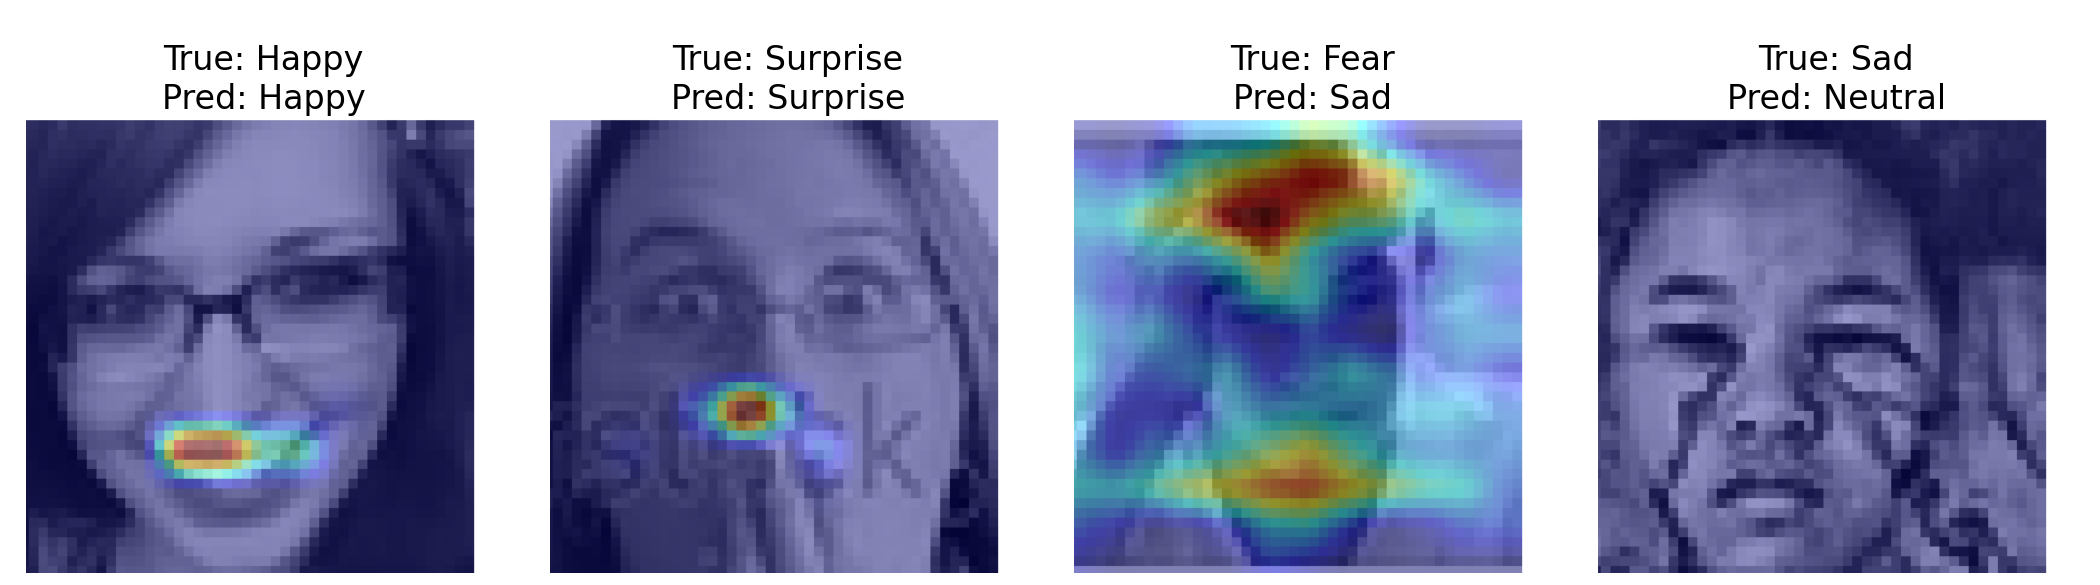
\includegraphics[width=\columnwidth]{results/step3_result/figures/gradcam_selected_examples_compact_row.png}
\caption{Grad-CAM examples for selected correct and incorrect CNN predictions.}
\label{fig:gradcam_examples}
\end{figure}

\section{Conclusion}

This project implemented a four-step facial emotion recognition pipeline:
dataset analysis, traditional ML baselines, CNN baseline training, and
ML-enhanced CNN analysis. The traditional ML experiments show that HOG is much
more effective than raw pixels and that HOG + KNN is the strongest traditional
baseline. The CNN baseline improves performance substantially, reaching a test
macro F1 of 0.5893. The final ML-enhanced CNN experiments show that traditional
ML can complement CNN predictions, especially through probability-level fusion
and stacking. The best hybrid model improves test macro F1 from 0.5893 for the
standalone CNN to 0.6078, corresponding to an absolute gain of 0.0185.
However, the improvement is moderate and the model still struggles with
visually similar or underrepresented emotions, especially Disgust, Fear, Sad,
and Neutral.

Overall, the project demonstrates that traditional ML methods are useful not
only as baselines, but also as complementary decision-level components for CNN
predictions. CNNs provide strong learned representations, while traditional ML
contributes feature analysis, decision-level fusion, and interpretable
correction strategies. Future work can
further improve the project by tuning the correction mechanism, exploring more
compact CNN architectures, applying stronger calibration methods, and testing
the approach on larger in-the-wild FER datasets such as
AffectNet~\cite{mollahosseini2019affectnet}.

\begin{thebibliography}{00}

\bibitem{goodfellow2013challenges}
I. J. Goodfellow, D. Erhan, P. L. Carrier, A. Courville, M. Mirza,
B. Hamner, W. Cukierski, Y. Tang, D. Thaler, D.-H. Lee, Y. Zhou,
C. Ramaiah, F. Feng, R. Li, X. Wang, D. Athanasakis, J. Shawe-Taylor,
M. Milakov, J. Park, R. Ionescu, M. Popescu, C. Grozea, J. Bergstra,
J. Xie, L. Romaszko, B. Xu, Z. Chuang, and Y. Bengio,
``Challenges in representation learning: A report on three machine learning
contests,'' \emph{Neural Networks}, vol. 64, pp. 59--63, 2015.

\bibitem{li2020deepfer}
S. Li and W. Deng, ``Deep facial expression recognition: A survey,''
\emph{IEEE Transactions on Affective Computing}, vol. 13, no. 3,
pp. 1195--1215, 2022.

\bibitem{dalal2005hog}
N. Dalal and B. Triggs, ``Histograms of oriented gradients for human
detection,'' in \emph{Proc. IEEE Conf. Computer Vision and Pattern Recognition
(CVPR)}, 2005, pp. 886--893.

\bibitem{wolpert1992stacked}
D. H. Wolpert, ``Stacked generalization,'' \emph{Neural Networks}, vol. 5,
no. 2, pp. 241--259, 1992.

\bibitem{selvaraju2017gradcam}
R. R. Selvaraju, M. Cogswell, A. Das, R. Vedantam, D. Parikh, and D. Batra,
``Grad-CAM: Visual explanations from deep networks via gradient-based
localization,'' in \emph{Proc. IEEE Int. Conf. Computer Vision (ICCV)}, 2017,
pp. 618--626.

\bibitem{mollahosseini2019affectnet}
A. Mollahosseini, B. Hasani, and M. H. Mahoor, ``AffectNet: A database for
facial expression, valence, and arousal computing in the wild,''
\emph{IEEE Transactions on Affective Computing}, vol. 10, no. 1, pp. 18--31,
2019.

\end{thebibliography}

\end{document}
